\documentclass{beamer}	
\mode<presentation>
 
\usepackage{pdfpages}
\usepackage{fancyvrb}
\usepackage{chemarr}

\usepackage{amsmath}		%% mathematics typesetting
\usepackage{amssymb}
 
\usepackage{ulem}

\usepackage{booktabs}

\usepackage{siunitx} %% tpyeset SI units

\usepackage{CJKutf8} %% typeset Chinese characters

\usepackage{pdfpages}

% Color and Theme. Can be changed. However, this one's quite nice.
\usetheme{Madrid}
\definecolor{theme}{rgb}{0.84,0,0.21}
\usecolortheme[named=theme]{structure}


%%  Title information
\title[Literatur-Recherche]{Wie erfahre ich von medizinischer Forschung? \\
Einführung in die Literatur-Recherche}
\author[melanie.stefan@medicalschool-berlin.de]{M14 Wissenschaftliches Arbeiten}
\institute[]{Prof. Melanie Stefan - melanie.stefan@medicalschool-berlin.de}
\date{WiSe 2023/24}
 

% Table of contents to pop up at the beginning of each section
\AtBeginSection[]
{
  \begin{frame}<beamer>
    \frametitle{Outline}
    \tableofcontents[currentsection,currentsubsection]
  \end{frame}
}
 
\beamertemplatenavigationsymbolsempty

\begin{document}
 
 
 
{ \usebackgroundtemplate{
\includegraphics[width=1.2\paperwidth]{MSB_Titelseite.pdf}} 
\begin{frame}

 \maketitle 

$\,$\\[6cm] 


\end{frame} 
}



 
%% Hook
\begin{frame}{Sie wissen, wie man wissenschaftliche Literatur liest\dots}

\begin{center}
    \includegraphics[width=\textwidth]{annie-spratt-CV3nkG7XIwg-unsplash.jpg}
\end{center}

    
\end{frame}


\begin{frame}{Aber wo finden?}

\begin{center}
    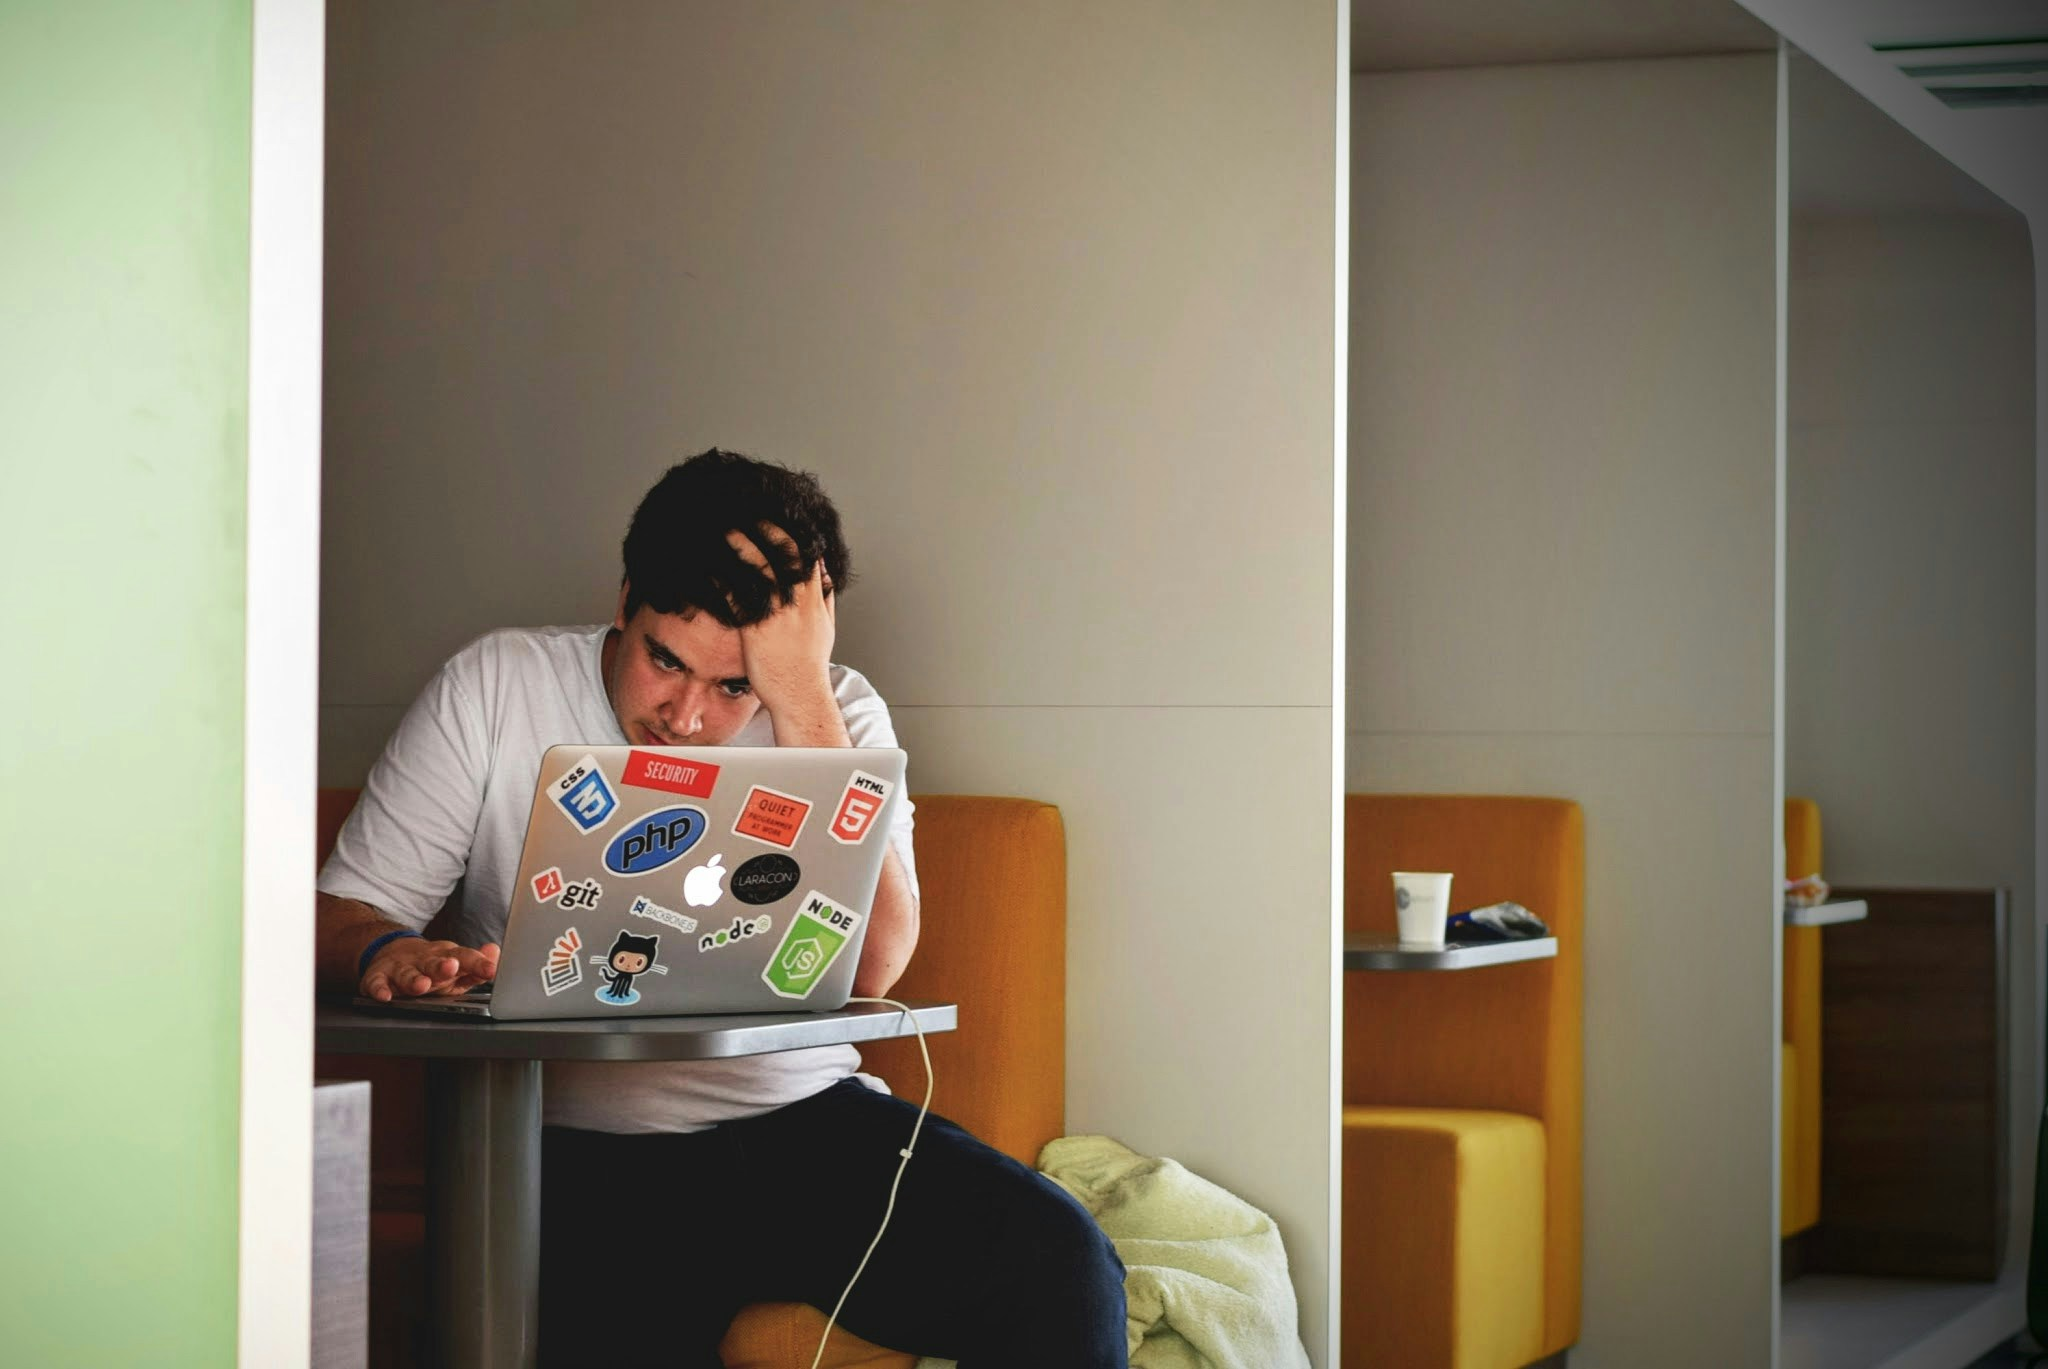
\includegraphics[width=\textwidth]{tim-gouw-1K9T5YiZ2WU-unsplash.jpg}
\end{center}

    
\end{frame}


%% TLIA
\begin{frame}
\frametitle{In dieser Vorlesung geht es um \dots}

\dots wissenschaftliche Information, wie sie geteilt wird, und wie wir sie gezielt suchen und finden können.

\begin{center}
    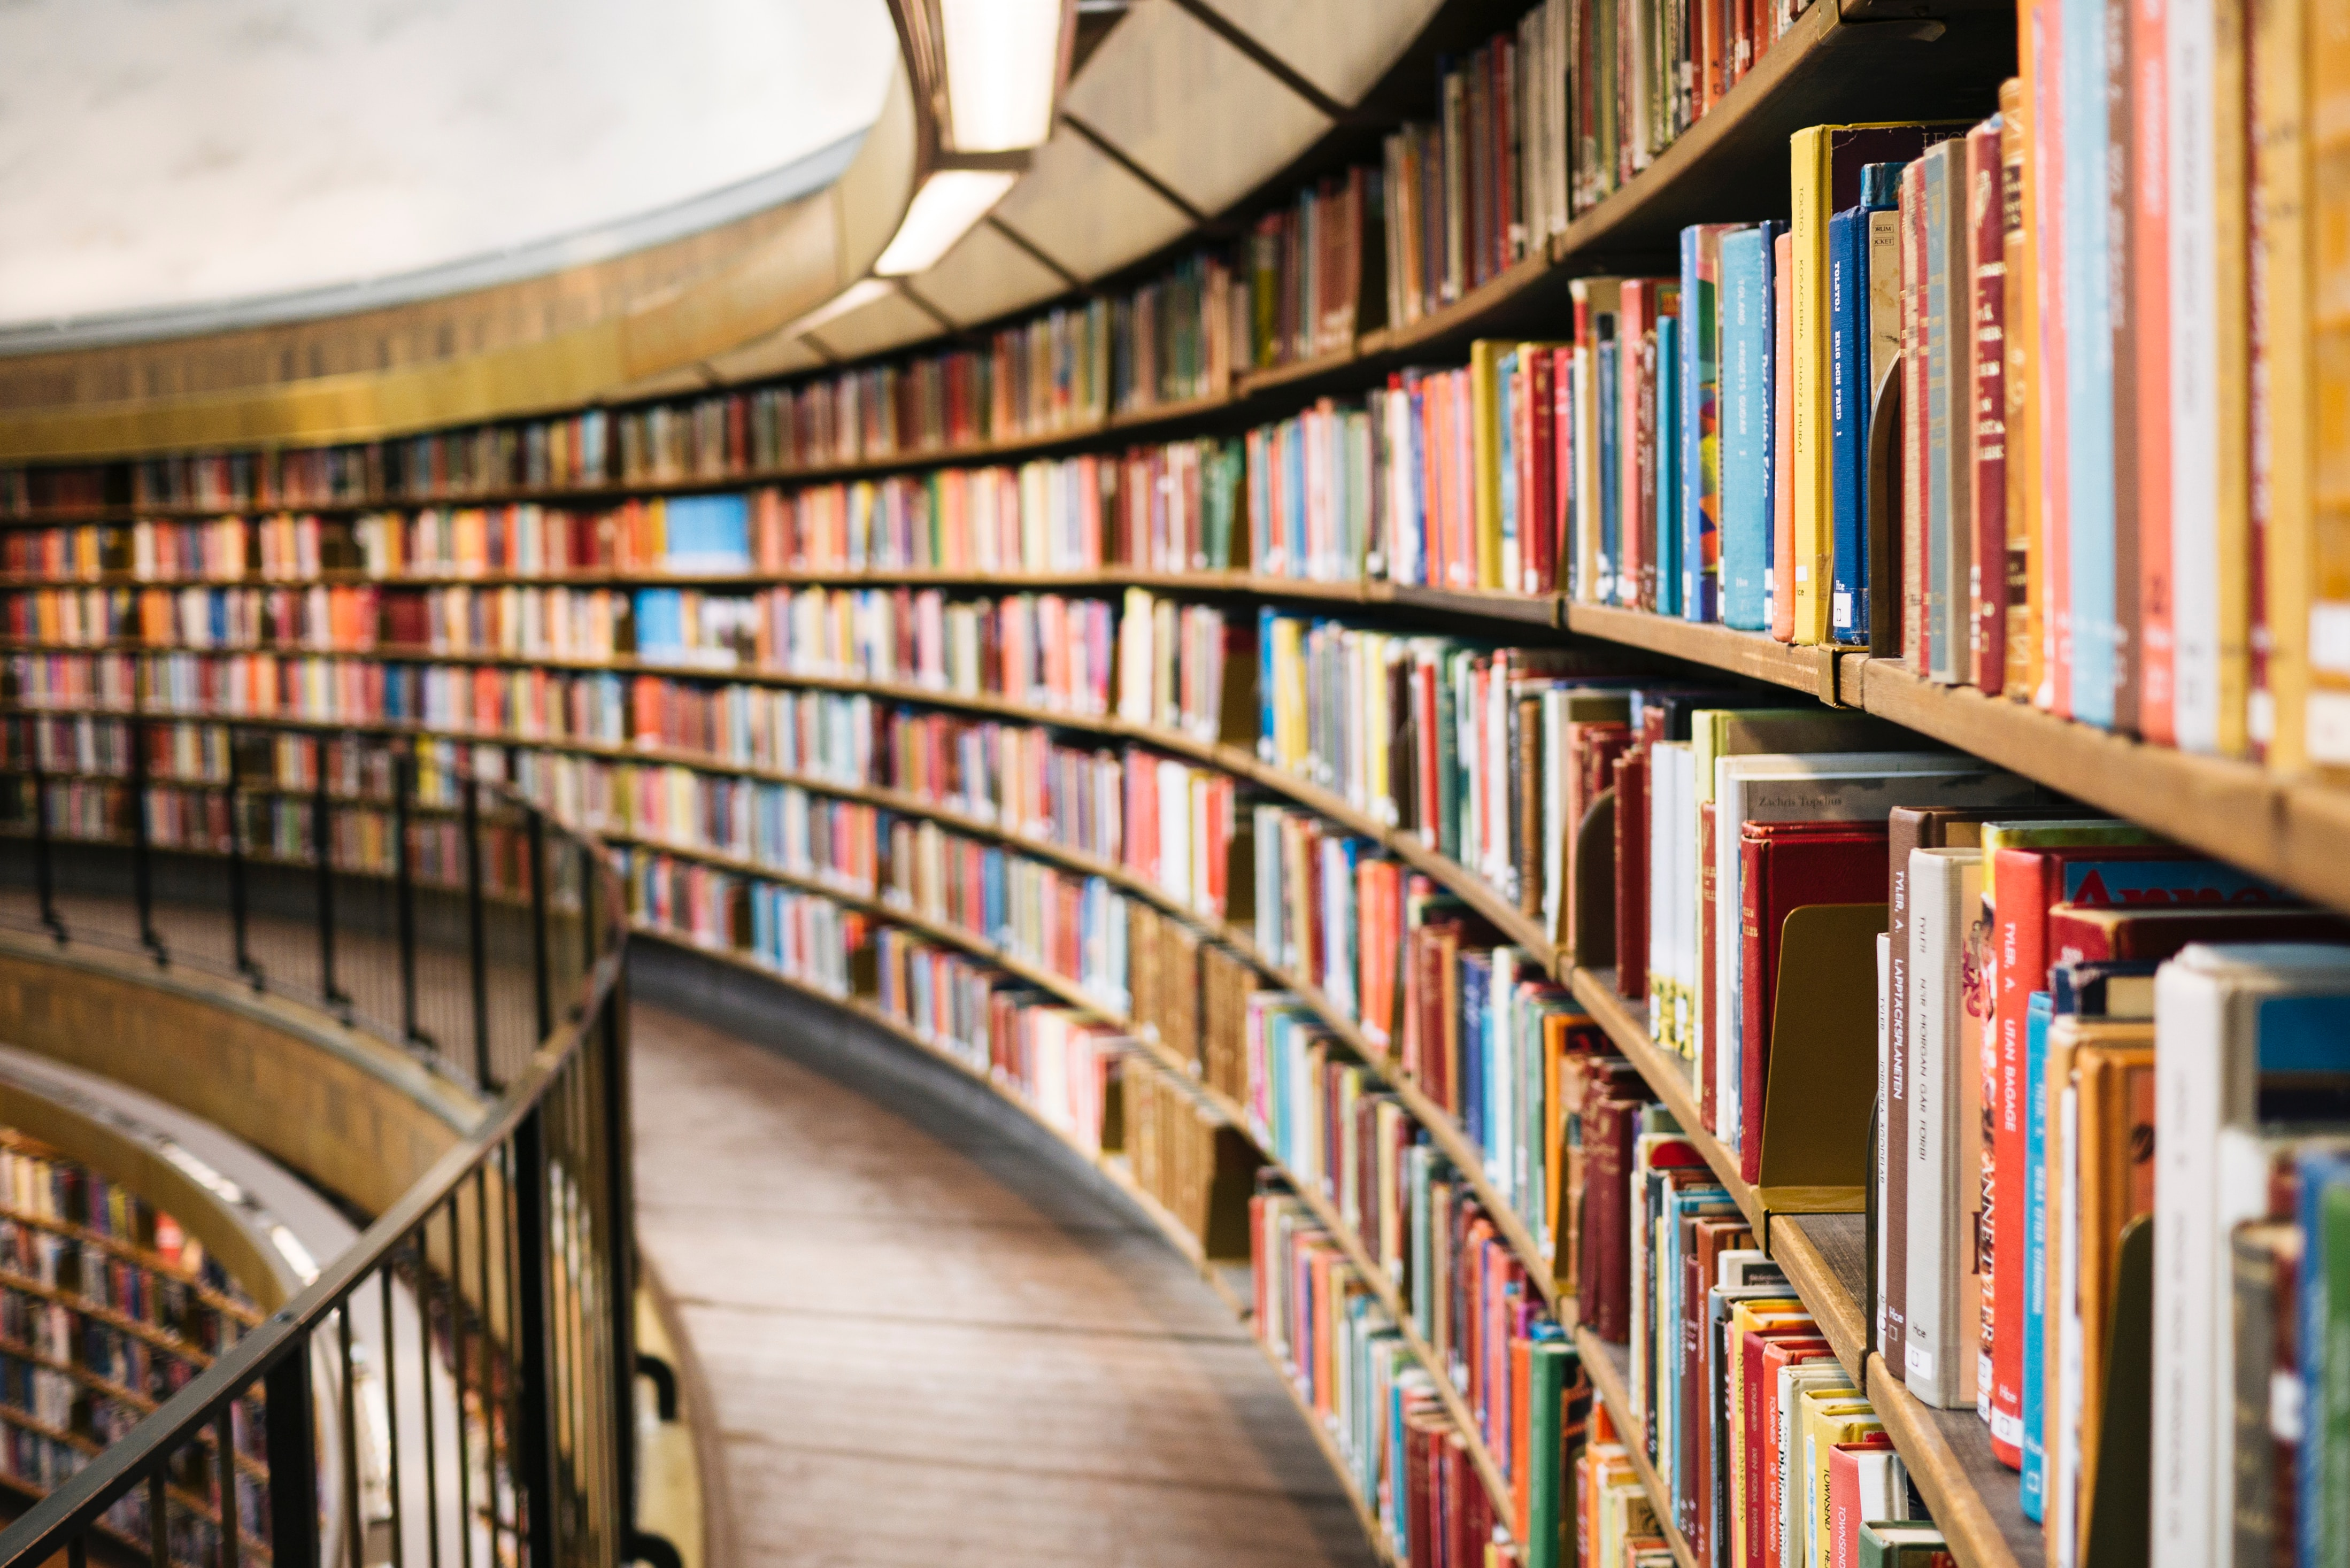
\includegraphics[width=0.7\textwidth]{susan-q-yin-2JIvboGLeho-unsplash.jpg}
\end{center}


 
\end{frame}



%% Learning Objectives

\begin{frame}

\frametitle{Nach dieser Vorlesung sollten Sie \dots}


\begin{itemize}
\item
Wissen, was die Bibliothek der MSB zu bieten hat
\item 
Medizinisch relevante Information finden
\item 
Medizinische Informationsquellen kritisch bewerten
\item 
Mehrere Wege kennen, um Zugang zu Büchern zu bekommen
\item 
Erklären, wie medizinische Forschungsergebnisse kommuniziert und publiziert werden
\item 
Verschiedene Datenbanken und Tools zur Literaturrecherche kennen und deren Vor- und Nachteile aufzählen
\item 
Strategien der Literaturrecherche aufzählen und vergleichen
\item 
Gezielt nach Literatur suchen
\item 
MeSH Terms und Boolean Operators bei der Literaturrecherche verwenden
\item 
Gefundene Literatur sammeln und verwalten
\end{itemize}

\end{frame}

%% Main Body


\section{Woher bekomme ich medizinische Information? }

\begin{frame}{Was sind Ihre Quellen, wenn Sie Information über ein medizinisches Thema brauchen?}

\pause

Häufig genutzte Quellen:

 \begin{itemize}
     \item 
Bücher
\item 
Zeitschriften
\item      
Lernplattformen wie AMBOSS, Via Medici, \dots
     \item 
     Wikipedia
     \item 
     \dots
 \end{itemize}

\end{frame}

\begin{frame}{Die Bibliothek kann mehr als Sie denken!}

\begin{columns}[c]
    \begin{column}{5cm}
    \begin{center}
    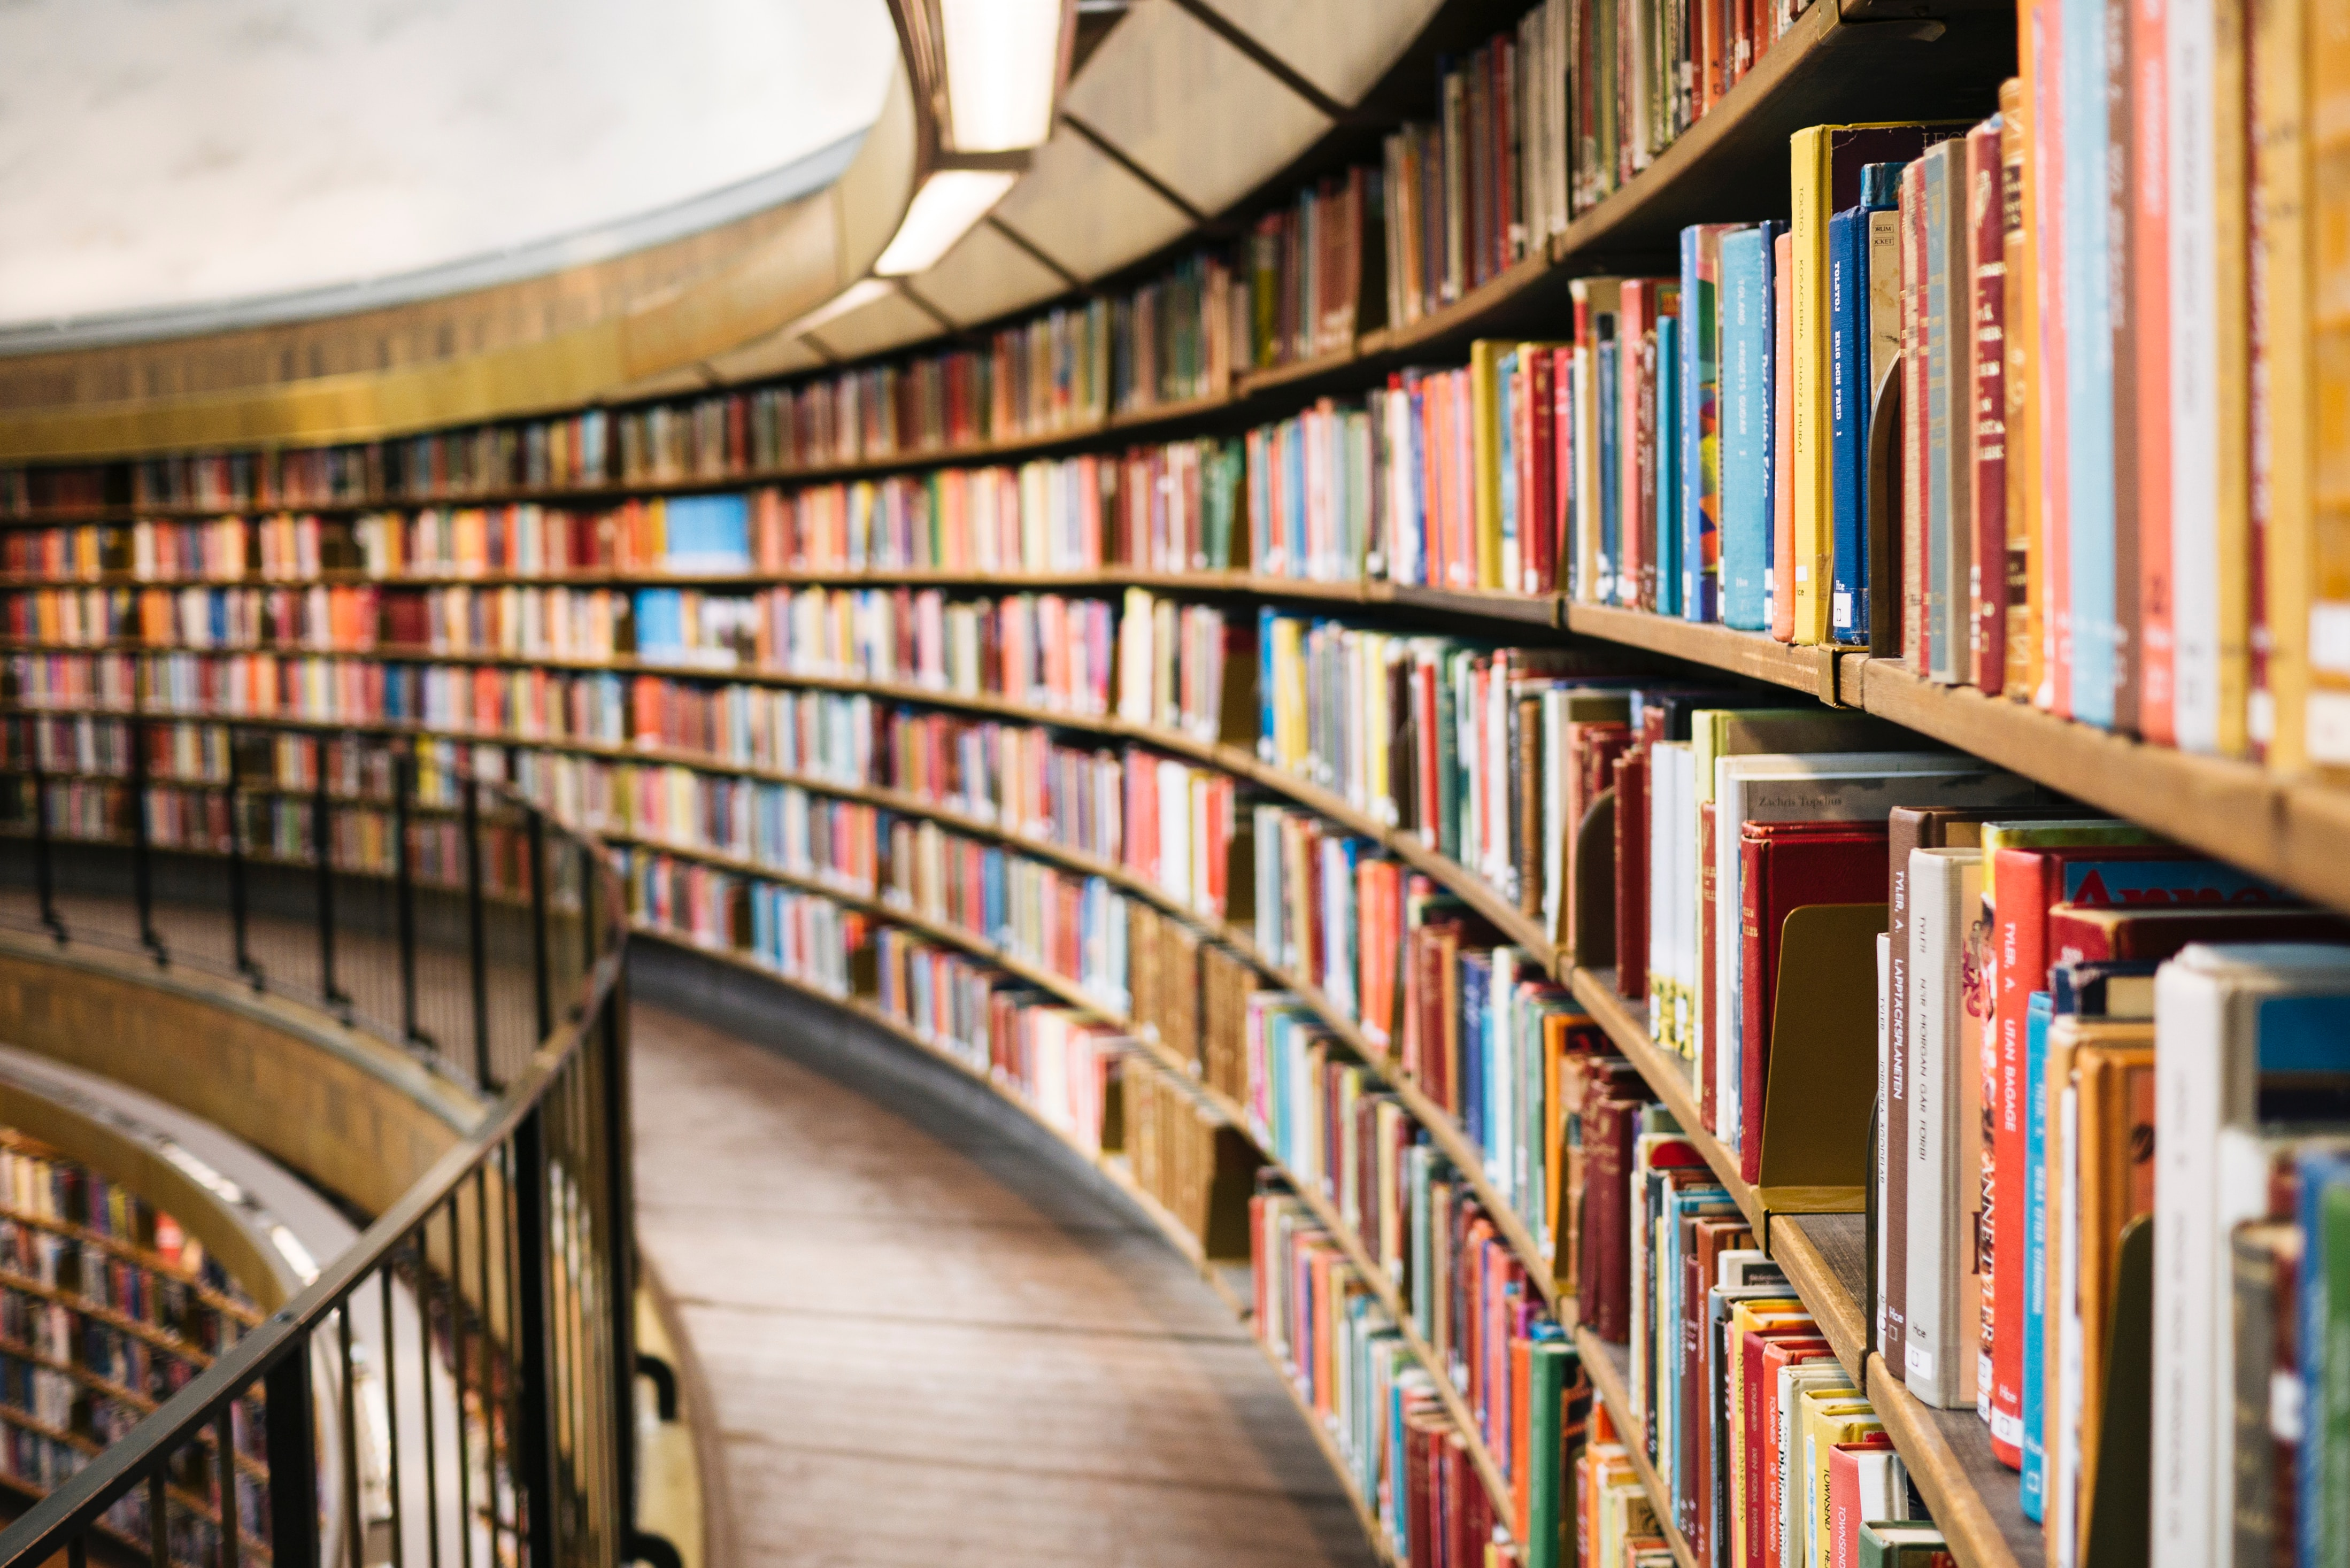
\includegraphics[width=\textwidth]{susan-q-yin-2JIvboGLeho-unsplash.jpg}
\end{center}

    \end{column}
        \begin{column}{7cm}
\begin{itemize}
    \item 
Lesen und Arbeiten vor Ort
\item 
Ausleihen von Büchern
\item 
    Zugang zu Zeitschriften, e-Books, Lernplattformen und Datenbanken online
    \item 
    Training zu Literaturrecherche und wissenschaftlichem Arbeiten
    \item 
    Fachleute für Information und Recherche
\end{itemize}
        
    \end{column}

\end{columns}

\end{frame}


\begin{frame}{Die Bibliothek der MSB}

\begin{block}{Ressourcen}
\begin{itemize}(
    \item 
    Online-Katalog der MSB: \url{https://www.eopac.net/BGX431775/}
    \item 
    Ausführliche Informationen zur Bibliothek im Trainex unter "Studiengang" (oder "Lernen") \(\rightarrow\) "Archiv(e)" \(\rightarrow\) "Zur Bibliothek"
\end{itemize} 
\end{block}

\begin{block}{Aufgabe (jetzt):}

Su

\end{block}

\end{frame}
% - Bib
% - Via Medici etc.
% - Wikipedia
% - Bücher
% - online portale
% -chatgpt

% %% Online Quellen
%  \begin{frame}
% \frametitle{Weitere Quellen}

% \begin{itemize}
% \item 
% Via Medici (nicht immer korrekt!)
% \item
% Formelsammlungen (am besten selber zusammenstellen)
% \item 
% Wikipedia: oft guter Überblick und nützliche weiterführende Quellen. Ersetzt aber nicht das Lehrbuch. 
% \end{itemize}


% \end{frame}


%  \begin{frame}
% \frametitle{Was ist mit ChatGPT?}

% \pause 

% \includegraphics[width=0.9\textwidth]{chatgpt_geographie_frage.png}

% \vfill
% \end{frame}


%  \begin{frame}
% \frametitle{ChatGPT ist eine Sprachmaschine, keine Faktenmaschine!}


% \includegraphics[width=0.9\textwidth]{chatgpt_geographie.png}

% \end{frame}


\section{Wie wird medizinische Forschung kommuniziert und publiziert?}

\begin{frame}{Wie werden wissenschaftliche Erkenntnisse publik gemacht?}

\begin{columns}[c]
    \begin{column}{5cm}
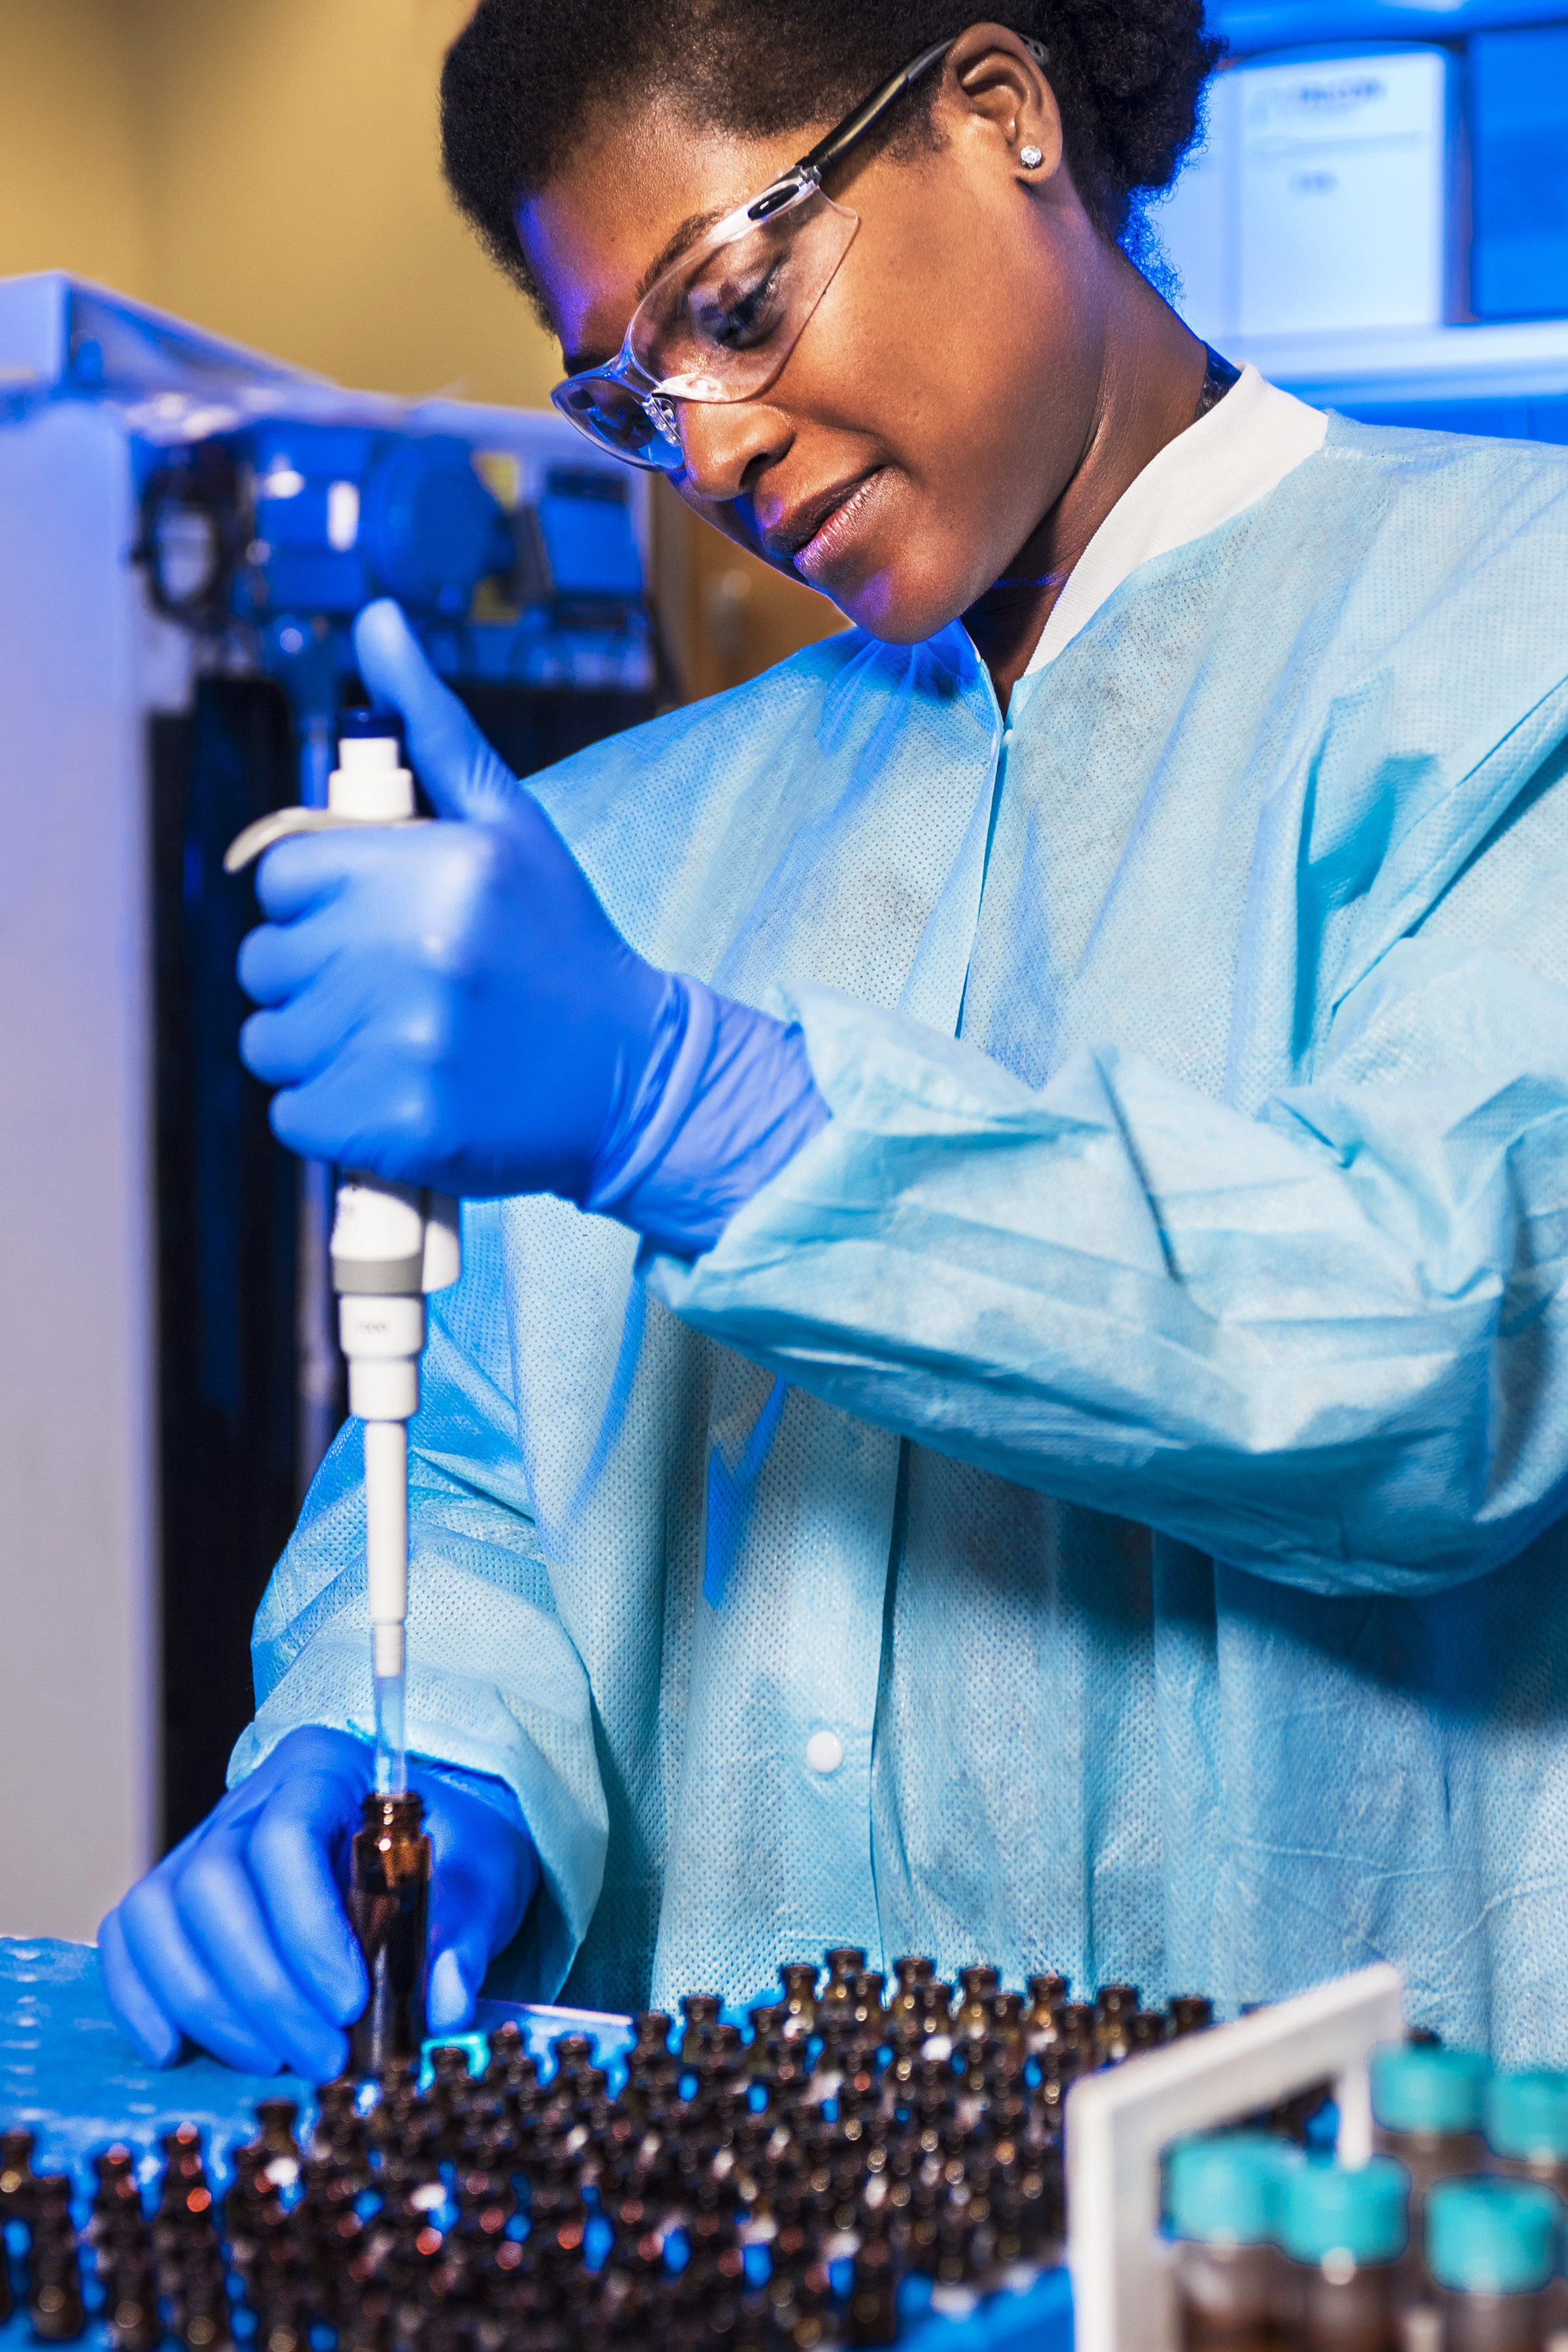
\includegraphics[width=\textwidth]{cdc-_N7I1JyPYJw-unsplash.jpg}        
    \end{column}
\pause
        \begin{column}{7cm}
        \begin{itemize}
            \item 
            Artikel in Fachzeitschriften
                    \item 
            Vorträge, Poster auf Fachtagungen
            \item 
            Bücher, technische Berichte, \dots 
            \item 
            Patente
            \item
            Deposition von Daten in spezifischen Datenbanken (z.B. für DNA-Sequenzen, Proteinstrukturen, Computermodelle, \dots)
            \item 
            Pressearbeit
            \item 
            Soziale Medien
            \item 
            \dots
        \end{itemize}
    \end{column}

\end{columns}
    
\end{frame}

\begin{frame}{Wie werden wissenschaftliche Erkenntnisse publik gemacht?}

\begin{columns}[c]
    \begin{column}{5cm}
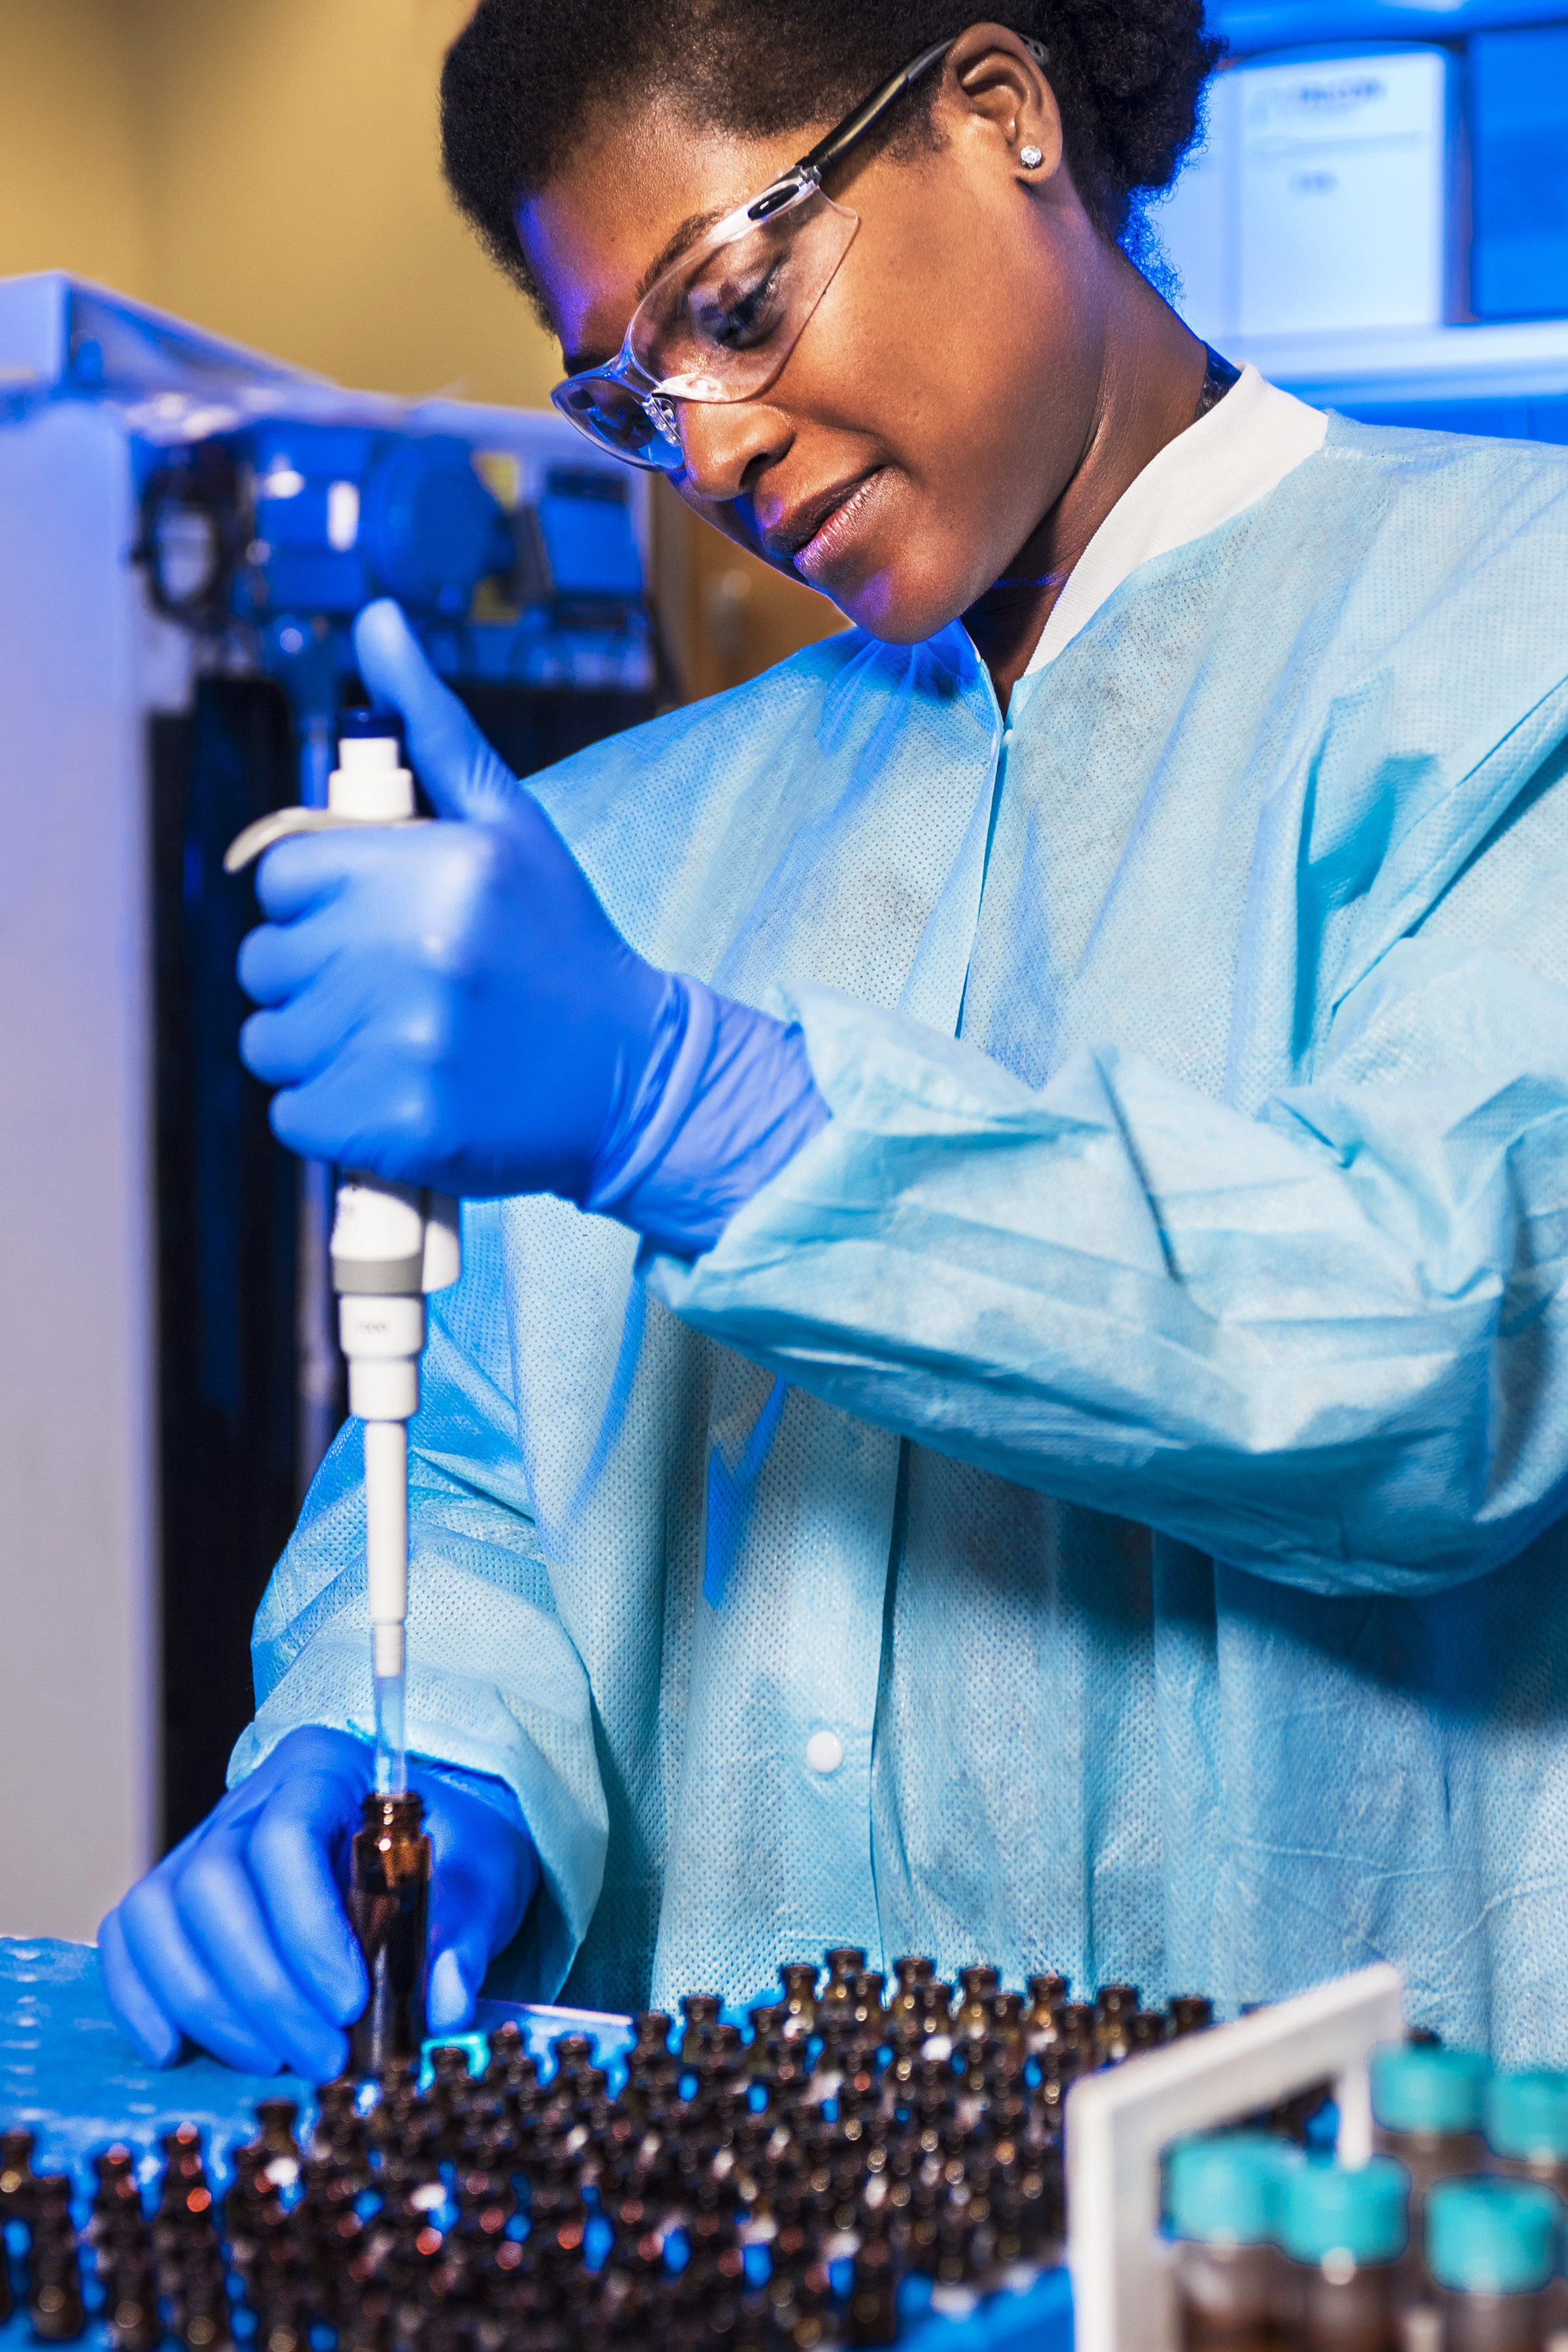
\includegraphics[width=\textwidth]{cdc-_N7I1JyPYJw-unsplash.jpg}        
    \end{column}
        \begin{column}{7cm}
        \begin{itemize}
            \item 
            \textbf{Artikel in Fachzeitschriften}
            \item 
            Vorträge, Poster auf Fachtagungen
            \item 
            Bücher, technische Berichte, \dots 
            \item 
            Patente
            \item 
            Deposition von Daten in spezifischen Datenbanken (z.B. für DNA-Sequenzen, Proteinstrukturen, Computermodelle, \dots)
            \item 
            Pressearbeit
            \item 
            Soziale Medien
 \item 
            \dots
        \end{itemize}
    \end{column}

\end{columns}
    
\end{frame}

% \begin{frame}{Artikel in wissenschaftlichen Fachzeitschriften}

% \begin{itemize}
%     \item 
% Zwischen 1 und ca. 5\,000 Autor*innen\footnote{Ja, ehrlich! Zum Beispiel: \url{https://journals.aps.org/prl/abstract/10.1103/PhysRevLett.114.191803}}. 
% \item 
% Artikel ist ein Bericht über Hintergründe, Methodik, Ergebnisse und kritische Evaluation einer wissenschaftlichen Studie 
% \item 
% Verschiedene Fachzeitschriften existieren für verschiedene Felder
% \item 


% \end{itemize}


% \end{frame}
%% peer review

%% Wer bezahlt? 

%% 

\section{Wie kann ich wissenschaftliche Literatur finden?}

\begin{frame}{Fallstudie: Kognitive Leistung im Alter}

Sie beginnen Ihre Doktorarbeit in einem Labor, das den Rückgang der kognitiven Leistung im Alter untersucht. Zuallererst wüssten Sie gerne mehr über das Altern. Wo finden Sie wissenschaftliche Literatur dazu?


\begin{center}
    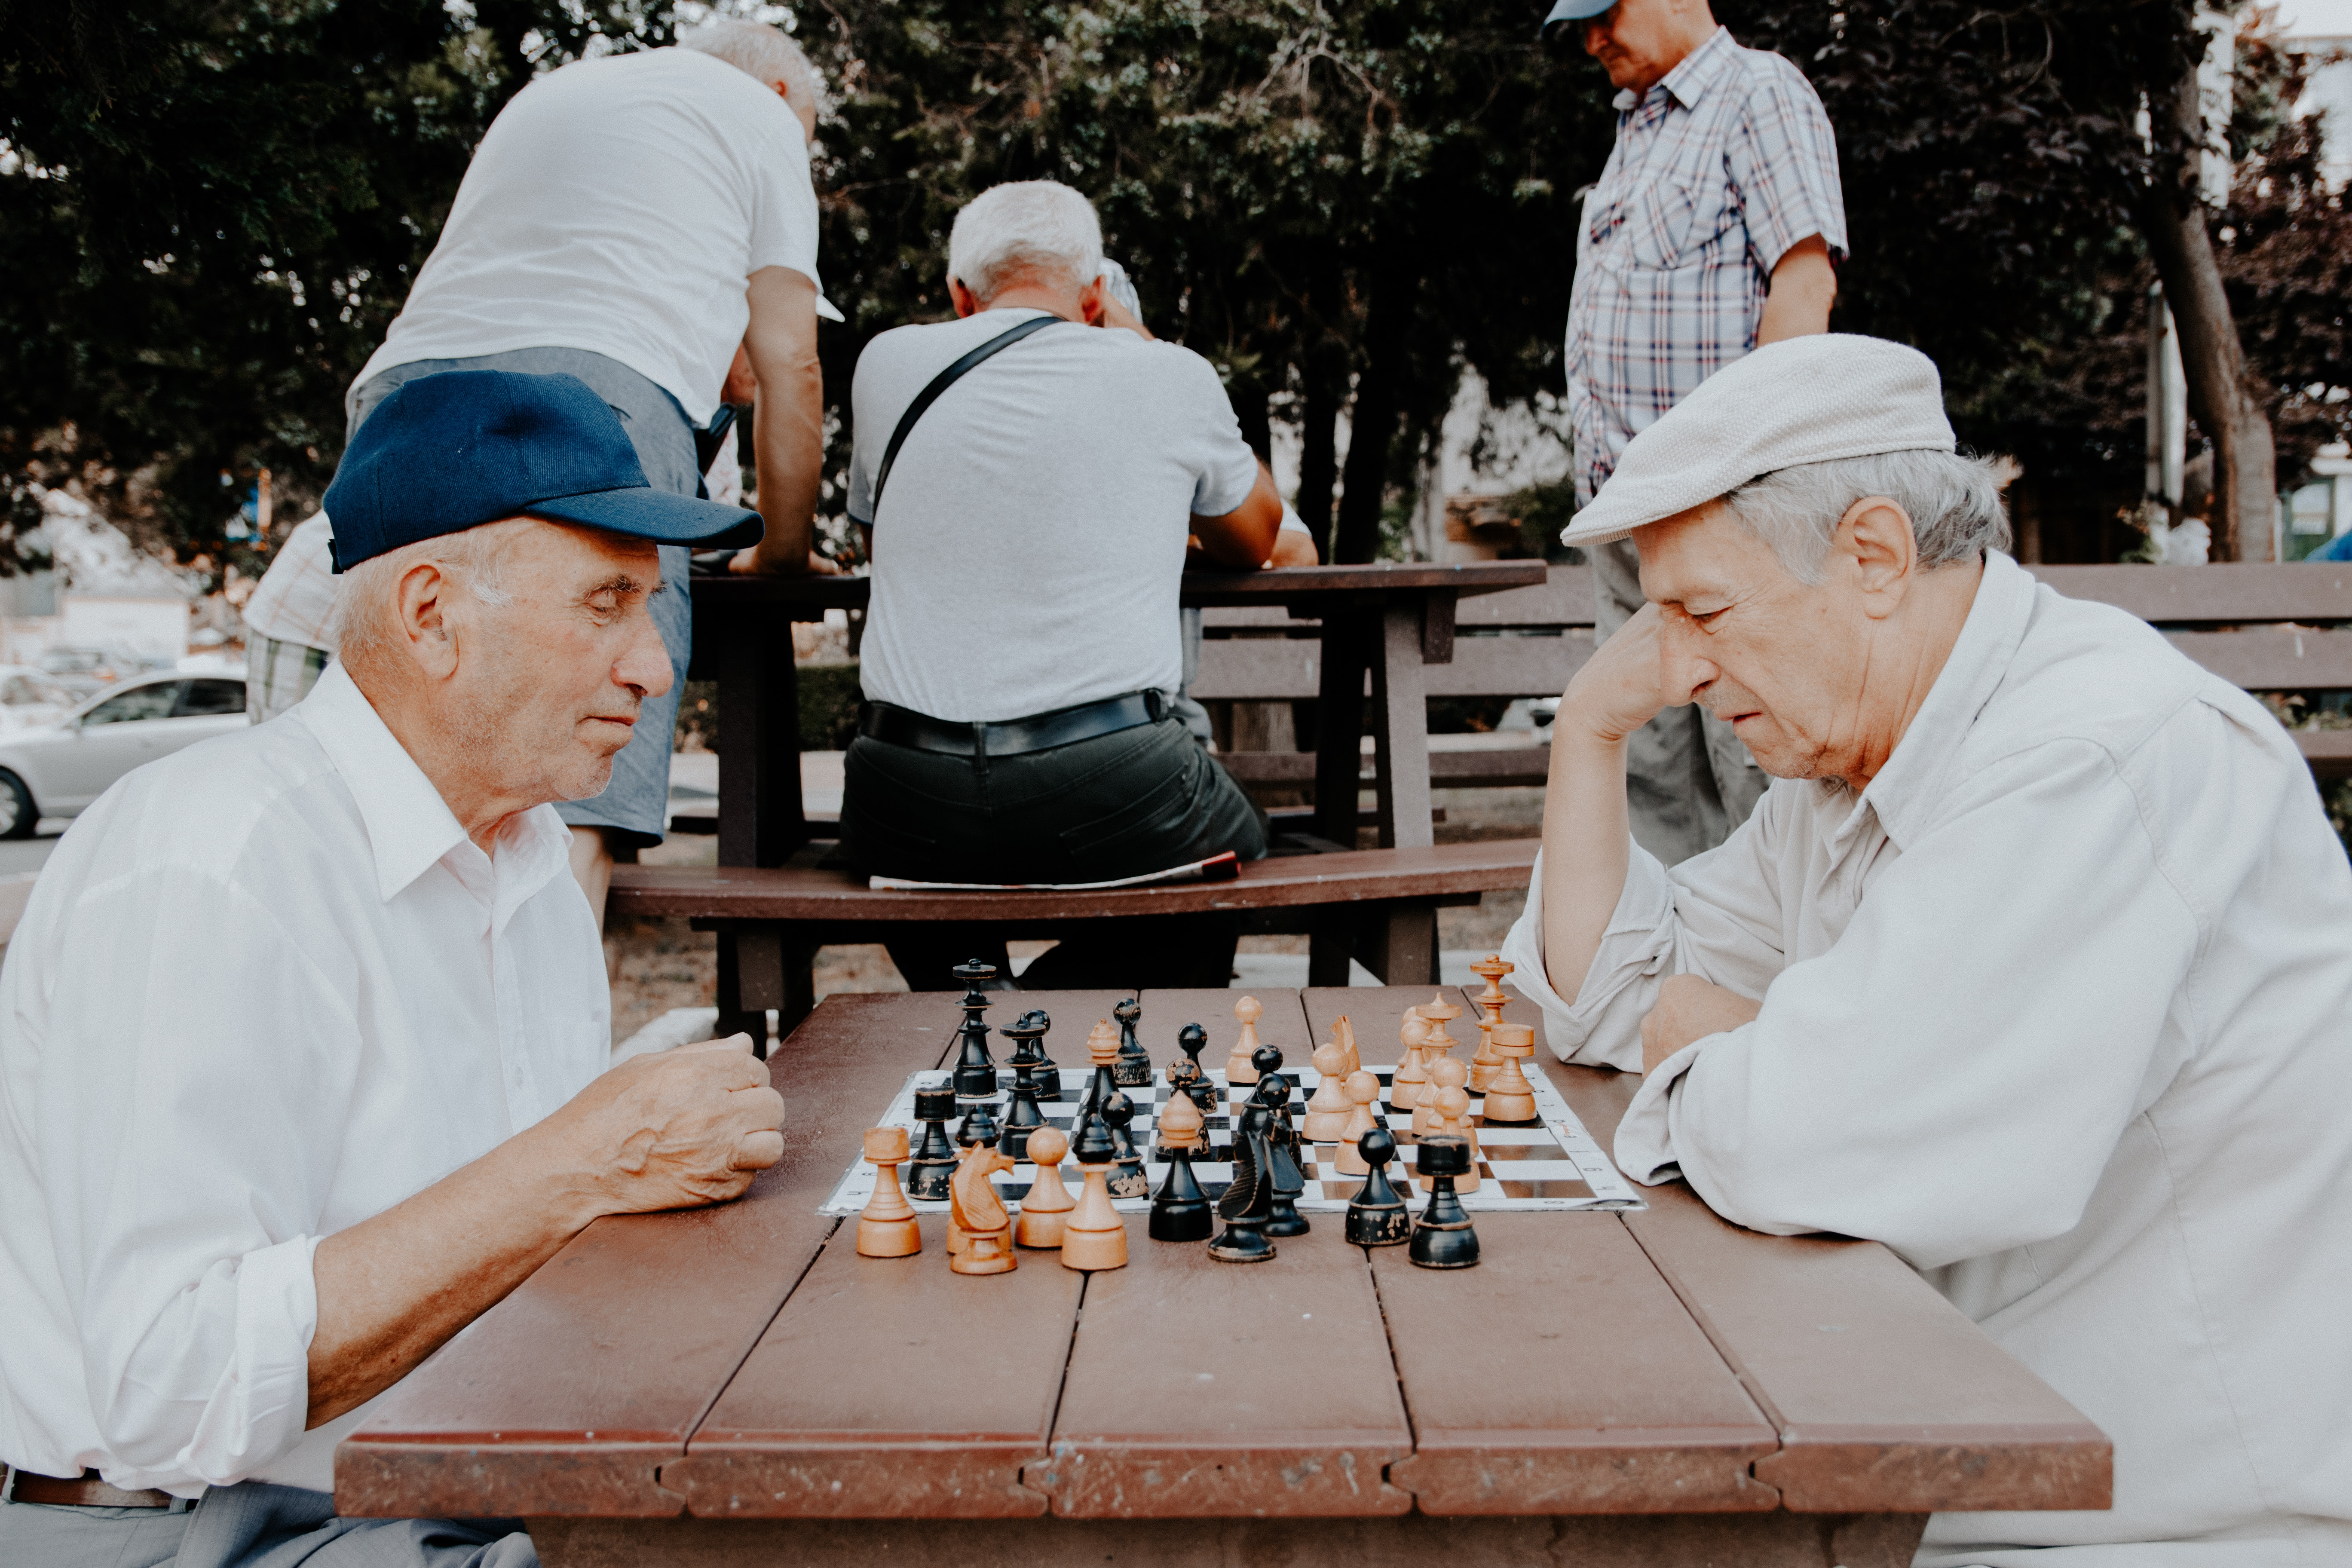
\includegraphics[width=0.5\textwidth]{vlad-sargu-ItphH2lGzuI-unsplash.jpg}
\end{center}



\end{frame}


\begin{frame}{Wissenschaftliche Literaturdatenbanken}

\begin{itemize}
    \item 
    Es gibt verschiedene Datenbanken, die wissenschaftliche Literatur sammeln und zur Verfügung stellen
    \item 
    Dabei gibt es Datenbanken für einzelne Fachbereiche oder allgemeine Datenbanken
    \item 
    Suchprozesse funktionieren überall ähnlich
    \item 
    \textbf{Aber:} Was in einer Datenbank gespeichert wird und was als Antwort auf eine Suchanfrage priorisiert wird, hängt von der Datenbank ab
\end{itemize}
    
\end{frame}


\begin{frame}{Fallstudie: Kognitive Leistung im Alter}

Suchen Sie auf den folgenden zwei Portalen nach dem Stichwort "ageing".

\begin{itemize}
    \item 
PubMed: \url{https://pubmed.ncbi.nlm.nih.gov/}
\item 
Google Scholar: \url{https://scholar.google.de/}
\end{itemize}


Beantworten Sie folgende Fragen:

\begin{itemize}
    \item 
    Wieviele Ergebnisse bekommen Sie jeweils?
    \item 
    Wie sind die Ergebnisse geordet? Wie lassen sie sich ordnen?
    \item 
    Bekommen Sie dieselben Ergebnisse wie Ihr*e Sitznachbar*in?
    \item 
    Wie sind die gefundenen Treffer thematisch einzuordnen?
\end{itemize}

\end{frame}

\begin{frame}{Vergleich: PubMed/Google Scholar}

\begin{tabular}{|p{3cm}|p{4cm}|p{4cm}|}
\hline
                & \textbf{PubMed}                       & \textbf{Google Scholar} \\
\hline
Betrieben von   & National Library of Medicine  & Google \\
\hline
Inhalt          & biomedical sciences    & allgemein \\
\hline
Algorithmus zum Sortieren   & unklar, aber konsistent   & unklar, nicht konsistent (daher nicht standardisierbar) \\
\hline
Sortierung nach Datum       & möglich                   & möglich \\
\hline
\end{tabular}


\end{frame}

%% Booleans
%% MESH terms

%% pubmed google scholar biorxiv scihub
%% paywalls, scihub




\section{Was mache ich mit der gefundenen Literatur?}

\begin{frame}{Literatur gefunden, was nun?}

\pause

Lesen, eh klar. \pause Aber auch: Notizen machen, organisieren und verwalten.  \\

\emph{Machen Sie das bereits, und wenn ja, dann wie?}

    
\end{frame}

\begin{frame}{Methoden für Notizen}

\begin{itemize}
    \item 
Hervorhebungen und Notizen am Artikel
\item 
"Post-it" mit 3-5 wichtigsten Punkten auf erster Seite\footnote{Danke an Prof. Katsuyuki Yugi!}
    \item
    Note-taking App (z.B. Evernote, OneNote, Notion, \dots) - Welche genau Sie verwenden ist egal, suchen Sie sich etwas aus, womit Sie gut zurecht kommen. Vorteil: Durchsuchbar!
\end{itemize}

\begin{center}
    
\includegraphics[width=0.5\textwidth]{kelly-sikkema-QtSDRxvZHQc-unsplash.jpg}
\end{center}

\end{frame}


\begin{frame}{Literaturverwaltung}

\begin{itemize}
    \item 
    Programme zur Literaturverwaltung erlauben uns, unsere eigenen Literaturdatenbanken (z.B. zu Themen) anzulegen
    \item 
    Artikel (aber auch Bücher, Dissertationen etc.) können einfach importiert werden und müssen nicht händisch hinzugefügt werden
    \item 
    Einfaches und richtiges Exportieren von Zitaten und Literaturlisten in Textverarbeitungssysteme wie Word, OpenOffice oder LaTeX
\item 
Mehrere existieren: z.B. EndNote, Citavi, Zotero, etc. Auch hier: Es ist egal, was Sie verwenden, aber verwenden Sie etwas! \pause \textcolor{red}{Kleine Demo}
\end{itemize}


\end{frame}

%% Review


\begin{frame}

\frametitle{Jetzt* sollten Sie \dots}


\begin{itemize}
\item
Wissen, was die Bibliothek der MSB zu bieten hat
\item 
Medizinisch relevante Information finden
\item 
Medizinische Informationsquellen kritisch bewerten
\item 
Mehrere Wege kennen, um Zugang zu Büchern zu bekommen
\item 
Erklären, wie medizinische Forschungsergebnisse kommuniziert und publiziert werden
\item 
Verschiedene Datenbanken und Tools zur Literaturrecherche kennen und deren Vor- und Nachteile aufzählen
\item 
Strategien der Literaturrecherche aufzählen und vergleichen
\item 
Gezielt nach Literatur suchen
\item 
MeSH Terms und Boolean Operators bei der Literaturrecherche verwenden
\item 
Gefundene Literatur sammeln und verwalten
\end{itemize}

\end{frame}


\begin{frame}

\begin{center}
    
\includegraphics[width=0.7\textwidth]{feedback_QR.png}
\end{center}


\url{https://forms.office.com/e/2eqByuL7q2}

\end{frame}

%% Bildnachweis
\begin{frame}
\frametitle{Bildnachweis}


\begin{tiny}
 
\begin{itemize}

\item 
Bibliothek. Photo by \href{https://unsplash.com/@syinq?utm_content=creditCopyText&utm_medium=referral&utm_source=unsplash}{Susan Q Yin} on \href{https://unsplash.com/photos/books-on-brown-wooden-shelf-2JIvboGLeho?utm_content=creditCopyText&utm_medium=referral&utm_source=unsplash}{Unsplash}
  

\item 
Frau sitzt am Laptop und konzentriert sich. Photo by \href{https://unsplash.com/@anniespratt?utm_content=creditCopyText&utm_medium=referral&utm_source=unsplash}{Annie Spratt} on \href{https://unsplash.com/photos/woman-in-black-long-sleeve-shirt-using-macbook-air-on-brown-wooden-table-CV3nkG7XIwg?utm_content=creditCopyText&utm_medium=referral&utm_source=unsplash}{Unsplash}
  

  
\item
Logo der MSB. MSB Medical School Berlin, Public Domain, via Wikimedia Commons

\item 
Mann sitzt am Laptop und rauft sich die Haare. Photo by \href{https://unsplash.com/@punttim?utm_content=creditCopyText&utm_medium=referral&utm_source=unsplash}{Tim Gouw} on \href{https://unsplash.com/photos/man-wearing-white-top-using-macbook-1K9T5YiZ2WU?utm_content=creditCopyText&utm_medium=referral&utm_source=unsplash}{Unsplash}

\item 
Post-it Zettel und zwei Stife. Photo by \href{https://unsplash.com/@kellysikkema?utm_content=creditCopyText&utm_medium=referral&utm_source=unsplash}{Kelly Sikkema} on \href{https://unsplash.com/photos/red-marker-and-orange-pen-on-white-surface-QtSDRxvZHQc?utm_content=creditCopyText&utm_medium=referral&utm_source=unsplash}{Unsplash}
  

\item 
Wissenschaftlerin beim Pipettieren.  Photo by \href{https://unsplash.com/@cdc?utm_content=creditCopyText&utm_medium=referral&utm_source=unsplash}{CDC} on \href{https://unsplash.com/photos/woman-holding-brown-glass-_N7I1JyPYJw?utm_content=creditCopyText&utm_medium=referral&utm_source=unsplash}{Unsplash}

\item 
Zwei ältere Männer spielen Schach. Photo by \href{https://unsplash.com/@vladsargu?utm_content=creditCopyText&utm_medium=referral&utm_source=unsplash}{Vlad Sargu} on \href{https://unsplash.com/photos/two-men-playing-chess-ItphH2lGzuI?utm_content=creditCopyText&utm_medium=referral&utm_source=unsplash}{Unsplash}
   
\end{itemize}

\end{tiny}
\end{frame}












\end{document}




